% chapter1.tex
% !TEX root = ../main.tex
\newpage


\begin{center}
    {\large\textbf{CHƯƠNG 1: KHẢO SÁT, PHÂN TÍCH, THAM KHẢO}}
\end{center}

\onehalfspacing
\section*{1.1 Giới thiệu}

Để chuẩn bị cho quá trình thiết kế giao diện hệ thống đặt vé xe khách, nhóm nghiên cứu đã thực hiện một cuộc khảo sát thực tế kỹ lưỡng, kết hợp với việc tham khảo và phân tích các hệ thống đặt vé tương tự hiện có trên thị trường. 
Mục tiêu của hoạt động này là đánh giá chính xác nhu cầu thực tế của người dùng, bao gồm thói quen, hành vi sử dụng và các kỳ vọng đối với một giao diện thân thiện, hiệu quả. 
Đồng thời, nhóm đã nghiên cứu các xu hướng thiết kế giao diện hiện đại và các yếu tố công nghệ đang được áp dụng rộng rãi trong lĩnh vực này.
 Dựa trên dữ liệu thu thập được từ khảo sát, nhóm đã tiến hành phân tích chuyên sâu các yêu cầu chức năng và phi chức năng, từ đó xây dựng cơ sở cho việc đề xuất giải pháp thiết kế giao diện tối ưu. 
 Giải pháp này không chỉ đảm bảo sự phù hợp với mục tiêu của đề tài mà còn hướng đến việc mang lại trải nghiệm người dùng mượt mà, trực quan và hiệu quả, đáp ứng tốt các tiêu chí về tính tiện dụng và thẩm mỹ.

  \section*{1.2 Mục tiêu và phương pháp khảo sát}

 \subsection*{1.2.1 Mục tiêu khảo sát}
 Quá trình khảo sát được triển khai với mục tiêu thu thập dữ liệu thực tế về nhu cầu, thói quen và những khó khăn mà người dùng gặp phải khi sử dụng các hệ thống đặt vé xe khách trực tuyến hiện nay. Mục đích chính là xác định các vấn đề cốt lõi trong trải nghiệm người dùng (UX), đồng thời làm rõ các yếu tố thiết kế cần được ưu tiên cải thiện để phát triển một giao diện web thân thiện, hiệu quả và phù hợp với kỳ vọng của người dùng. 

Cụ thể, khảo sát tập trung vào việc giải đáp các câu hỏi trọng tâm sau: 
\begin{itemize}
    \item Người dùng thường sử dụng phương thức nào (trực tuyến, tại quầy, hoặc qua ứng dụng di động) để đặt vé xe khách?
    \item Những yếu tố nào trong các hệ thống hiện tại khiến người dùng cảm thấy hài lòng hoặc không hài lòng, chẳng hạn như tính dễ sử dụng, tốc độ xử lý, hay mức độ rõ ràng của thông tin?
    \item Người dùng kỳ vọng những đặc điểm gì ở một giao diện đặt vé lý tưởng, bao gồm bố cục, màu sắc, tính năng, và khả năng tương thích với thiết bị?
    \item Các thao tác nào được người dùng thực hiện thường xuyên nhất trong quá trình đặt vé, ví dụ như tìm kiếm chuyến xe, chọn ghế, hoặc thanh toán?
    \item Mức độ ưu tiên của người dùng đối với các yếu tố như tính tiện lợi, tốc độ tải trang, khả năng tra cứu thông tin nhanh chóng, và cách trình bày bố cục giao diện.
\end{itemize}


Dựa trên dữ liệu thu thập được, nhóm đã tiến hành phân tích chi tiết để xác định các điểm mạnh, điểm yếu của các hệ thống hiện có, từ đó đề xuất các giải pháp thiết kế giao diện tối ưu, đáp ứng tốt hơn nhu cầu thực tế và nâng cao trải nghiệm người dùng.

\subsection*{1.2.2 Phương pháp khảo sát}
% Mô tả mục tiêu và phương pháp khảo sát
Để đảm bảo tính đại diện và thu thập dữ liệu phù hợp với đối tượng mục tiêu của hệ thống đặt vé xe khách, nhóm đã triển khai phương pháp khảo sát trực tuyến thông qua biểu mẫu Google Forms. Phương pháp này được lựa chọn nhờ khả năng tiếp cận nhanh, tiết kiệm chi phí và hỗ trợ xử lý dữ liệu hiệu quả. Nội dung khảo sát được thiết kế kỹ lưỡng, kết hợp các câu hỏi đóng (trắc nghiệm một hoặc nhiều lựa chọn) để thu thập dữ liệu định lượng và câu hỏi mở để ghi nhận dữ liệu định tính, qua đó cung cấp cái nhìn toàn diện về nhu cầu, thói quen và kỳ vọng của người dùng đối với giao diện website đặt vé.

% Chi tiết các bước thực hiện khảo sát
Quá trình khảo sát được thực hiện theo các bước cụ thể như sau:
\begin{itemize}
    \item \textbf{Thiết kế bảng câu hỏi:} Nhóm đã xây dựng một biểu mẫu khảo sát với các câu hỏi được thiết kế cẩn thận, tập trung vào ba khía cạnh chính: thói quen sử dụng dịch vụ đặt vé xe khách (tần suất, phương thức đặt vé), mức độ hài lòng với các hệ thống hiện tại (về giao diện, tốc độ, tính tiện lợi), và kỳ vọng đối với giao diện website trong tương lai (bố cục, tính năng, trải nghiệm người dùng). Các câu hỏi được sắp xếp logic, dễ hiểu, và phù hợp với đối tượng người dùng mục tiêu.
    \item \textbf{Phát hành khảo sát:} Biểu mẫu được phân phối thông qua các kênh trực tuyến gồm mạng xã hội, email và các nhóm cộng đồng liên quan đến du lịch và di chuyển. Đối tượng khảo sát là những người dùng trong độ tuổi từ dưới 18 đến trên 50, bao gồm sinh viên, người đi làm và những người thường xuyên di chuyển liên tỉnh, nhằm đảm bảo tính đa dạng và phù hợp với nhóm người dùng chính của hệ thống.
    \item \textbf{Tổng hợp và phân tích dữ liệu:} Sau khi kết thúc giai đoạn thu thập, dữ liệu từ biểu mẫu được tổng hợp và xử lý bằng các công cụ thống kê như Google Sheets và phần mềm phân tích cơ bản. Dữ liệu định lượng được biểu diễn dưới dạng biểu đồ và số liệu thống kê để xác định xu hướng, trong khi dữ liệu định tính được phân loại và mã hóa để rút ra các đặc điểm hành vi, sở thích và vấn đề người dùng gặp phải, từ đó định hướng thiết kế giao diện.
\end{itemize}

% Đánh giá ưu điểm của phương pháp
Phương pháp khảo sát trực tuyến thông qua Google Forms cho phép nhóm thu thập dữ liệu một cách nhanh chóng, hiệu quả và tiết kiệm chi phí, đồng thời đảm bảo sự đa dạng trong đối tượng tham gia. Kết quả khảo sát cung cấp cơ sở dữ liệu đáng tin cậy, giúp nhóm nhận diện các điểm mạnh, điểm yếu của các hệ thống hiện tại và xác định các yếu tố thiết kế cần ưu tiên. Những thông tin này đóng vai trò quan trọng trong việc đề xuất giải pháp giao diện tối ưu, đáp ứng tốt các yêu cầu về tính tiện dụng, thẩm mỹ và trải nghiệm người dùng, đồng thời phù hợp với mục tiêu của đề tài.

\section*{1.3 Đối tượng và nội dung khảo sát}

% Mô tả đối tượng khảo sát
\subsection*{1.3.1 Đối tượng khảo sát}
Để đảm bảo dữ liệu thu thập phản ánh đúng nhu cầu và trải nghiệm của người dùng mục tiêu, khảo sát được triển khai trực tuyến thông qua biểu mẫu Google Forms, hướng đến các đối tượng thường xuyên di chuyển liên tỉnh bằng xe khách. Cụ thể, đối tượng khảo sát bao gồm sinh viên, người lao động và các cá nhân có nhu cầu đi lại thường xuyên. Nhóm tuổi mục tiêu được xác định từ 18 đến 45 tuổi, tập trung chủ yếu vào người dùng trẻ, những người quen thuộc với công nghệ và đã có kinh nghiệm sử dụng các nền tảng đặt vé trực tuyến. 

Việc lựa chọn đối tượng khảo sát được dựa trên hai tiêu chí chính:
\begin{itemize}
    \item Người tham gia đã từng đặt vé xe khách, thông qua các phương thức trực tiếp tại quầy hoặc qua các nền tảng trực tuyến như ứng dụng di động hoặc website.
    \item Người tham gia có khả năng đánh giá và cung cấp ý kiến đóng góp về trải nghiệm giao diện người dùng, từ đó giúp nhóm hiểu rõ các vấn đề thực tế và kỳ vọng của họ đối với hệ thống.
\end{itemize}
Tổng số người tham gia khảo sát và các thông tin thống kê chi tiết sẽ được trình bày trong các phần tiếp theo của báo cáo.

% Mô tả nội dung khảo sát
\subsection*{1.3.2 Nội dung khảo sát}
Bảng khảo sát được thiết kế gồm 13 câu hỏi, kết hợp giữa câu hỏi đóng (trắc nghiệm đơn hoặc đa lựa chọn) và câu hỏi mở, được chia thành bốn nhóm nội dung chính nhằm thu thập dữ liệu toàn diện về hành vi, trải nghiệm và kỳ vọng của người dùng. Các nhóm nội dung bao gồm:

\begin{enumerate}
    \item \textbf{Thông tin nhân khẩu học và hành vi di chuyển:}
    \begin{itemize}
        \item Bạn thuộc nhóm tuổi nào?
        \item Bạn đang sinh sống tại khu vực nào (thành phố, nông thôn, v.v.)?
        \item Bạn thường sử dụng phương tiện nào để di chuyển liên tỉnh (xe khách, tàu hỏa, máy bay, v.v.)?
        \item Bạn thường đi xe khách với mục đích gì (du lịch, công tác, về quê, v.v.)?
    \end{itemize}
    Nhóm câu hỏi này nhằm thu thập thông tin cơ bản về đặc điểm nhân khẩu học và thói quen di chuyển của người dùng, từ đó xác định đối tượng sử dụng chính của hệ thống.

    \item \textbf{Trải nghiệm sử dụng ứng dụng đặt vé:}
    \begin{itemize}
        \item Bạn đã từng sử dụng ứng dụng hoặc website đặt vé xe khách nào chưa?
        \item Bạn đã sử dụng những nền tảng đặt vé nào (tên cụ thể)?
        \item Bạn đánh giá trải nghiệm đặt vé trên các nền tảng đó như thế nào (dễ sử dụng, tốc độ, độ tin cậy, v.v.)?
        \item Bạn đã gặp phải những khó khăn nào khi sử dụng các nền tảng đặt vé trực tuyến?
    \end{itemize}
    Nhóm câu hỏi này tập trung đánh giá trải nghiệm thực tế của người dùng với các hệ thống hiện tại, nhằm nhận diện các vấn đề và hạn chế trong thiết kế giao diện.

    \item \textbf{Thói quen và yếu tố ảnh hưởng đến việc đặt vé:}
    \begin{itemize}
        \item Nếu bạn không sử dụng ứng dụng mà đặt vé trực tiếp, lý do là gì (thiếu tin tưởng, không tiện lợi, v.v.)?
        \item Yếu tố nào bạn cho là quan trọng nhất khi đặt vé trực tuyến (tốc độ, tính dễ sử dụng, giá cả, thông tin rõ ràng, v.v.)?
        \item Bạn thường sử dụng thiết bị nào để đặt vé (điện thoại, máy tính bảng, máy tính cá nhân)?
    \end{itemize}
    Nhóm câu hỏi này giúp nhóm hiểu rõ thói quen, ưu tiên và các yếu tố ảnh hưởng đến quyết định sử dụng dịch vụ đặt vé trực tuyến của người dùng.

    \item \textbf{Kỳ vọng và đề xuất từ người dùng:}
    \begin{itemize}
        \item Bạn mong muốn những tính năng nào có trong một ứng dụng hoặc website đặt vé xe khách?
        \item Bạn có đề xuất gì để cải thiện trải nghiệm sử dụng ứng dụng đặt vé xe khách?
    \end{itemize}
    Nhóm câu hỏi này tập trung thu thập ý kiến đóng góp và kỳ vọng của người dùng, từ đó định hướng các tính năng và cải tiến cần thiết cho giao diện hệ thống.
\end{enumerate}

% Nhấn mạnh ý nghĩa của cách thiết kế khảo sát
Việc tổ chức bảng khảo sát theo bốn nhóm nội dung trên giúp nhóm phân tích dữ liệu một cách có hệ thống, tập trung vào từng khía cạnh cụ thể của trải nghiệm người dùng, từ hành vi di chuyển, trải nghiệm thực tế, đến mong muốn cải tiến. Kết quả khảo sát cung cấp cơ sở dữ liệu quan trọng, làm nền tảng cho việc phân tích và đề xuất giải pháp thiết kế giao diện tối ưu, đáp ứng tốt các yêu cầu về tính tiện dụng, hiệu quả và sự phù hợp với người dùng Việt Nam.

% Mô tả tổng quan về quá trình thu thập và phân tích kết quả khảo sát
\subsection*{1.4 Kết quả khảo sát}
Sau khi triển khai biểu mẫu khảo sát trực tuyến trong vòng 5 ngày, nhóm đã thu thập được 112 phản hồi hợp lệ từ người dùng thuộc nhiều độ tuổi, khu vực và bối cảnh khác nhau. Dữ liệu được tổng hợp và phân tích kỹ lưỡng theo bốn nhóm nội dung chính, nhằm cung cấp cái nhìn toàn diện về hành vi, trải nghiệm và kỳ vọng của người dùng đối với hệ thống đặt vé xe khách trực tuyến. Các kết quả được trình bày chi tiết theo từng nhóm nội dung như sau:

% Kết quả về thông tin nhân khẩu học và hành vi di chuyển
\subsubsection{Thông tin nhân khẩu học và hành vi di chuyển}
\begin{itemize}
    \item \textbf{Độ tuổi:} Trong số tất cả người tham gia, 51.6\% thuộc nhóm tuổi từ 18 đến 25, 45.2\% từ 26 đến 35, và phần còn lại (3.2\%) là thuộc nhóm còn lại. Kết quả này cho thấy người dùng trẻ, đặc biệt là sinh viên và người lao động trẻ, là nhóm đối tượng chính sử dụng công nghệ để đặt vé xe khách.
    \item \textbf{Nơi sinh sống:} Gần 38.7\% người tham gia hiện đang sinh sống tại các thành phố lớn như Thành phố Hồ Chí Minh, Hà Nội và Đà Nẵng, nơi có hạ tầng mạng và thiết bị di động phát triển, tạo điều kiện thuận lợi cho việc sử dụng các nền tảng đặt vé trực tuyến.
    \item \textbf{Phương tiện di chuyển liên tỉnh:} Xe khách là phương tiện được 142\% người khảo sát lựa chọn thường xuyên (\textit{Lưu ý: Tỷ lệ này cao hơn 100\% vì người khảo sát có thể chọn nhiều hơn một loại xe khách.}), tiếp theo là máy bay (64.5\%) và xe máy cá nhân (35.5\%).
    \item \textbf{Mục đích di chuyển:} Về mục đích di chuyển, khoảng 61.3\% người tham gia cho biết họ thường đi xe khách để về quê, 29.0\% đi công tác, và 83.9\% di chuyển với mục đích du lịch. (Lưu ý: tổng tỷ lệ này cao hơn 100\% vì người khảo sát có thể chọn nhiều hơn một loại mục đích)
\end{itemize}
\begin{center}
    

\begin{figure}[h]
    \centering
    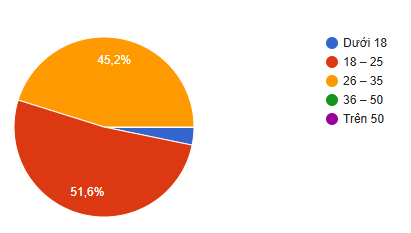
\includegraphics[width=0.6\textwidth]{assets/chart/1.4.1.png}
    \caption{\textit{Biểu đồ nhóm tuổi người tham gia khảo sát.}} \textit{Nhóm người trẻ (học sinh, sinh viên) chiếm đa số.}
    \label{fig:nhom_tuoi}
\end{figure}

\begin{figure}[h]
    \centering
    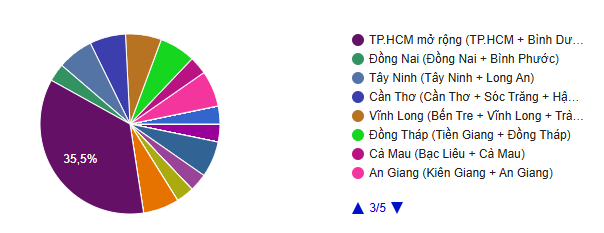
\includegraphics[width=1\textwidth]{assets/chart/1.4.2.png}
    \caption{\textit{Biểu đồ khu vực người tham gia khảo sát.}} \textit{Hơn 50\% là từ các thành phố lớn với hạ tầng công nghệ phát triển.}
    \label{fig:khu_vuc}
\end{figure}

\begin{figure}[h]
    \centering
    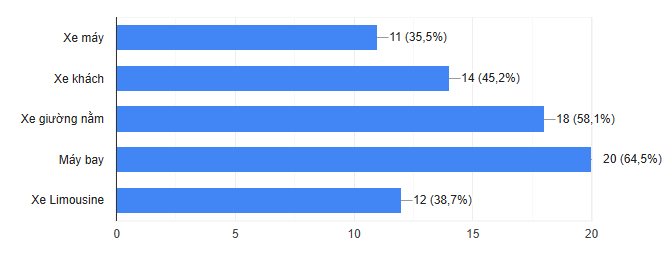
\includegraphics[width=0.8\textwidth]{assets/chart/1.4.3.png}
    \caption{\textit{Biểu đồ nhóm phương tiện di chuyển của người tham gia khảo sát.}} \textit{phương tiện chiếm đa số là xe khách.}
    \label{fig:nhom_phuong_tien}
\end{figure}

\begin{figure}[h]
    \centering
    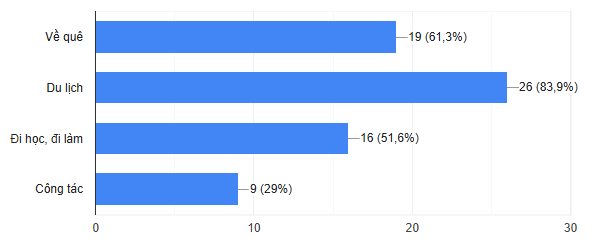
\includegraphics[width=0.6\textwidth]{assets/chart/1.4.4.png}
    \caption{\textit{Biểu đồ mục đích di chuyển của người tham gia khảo sát.}} \textit{Mục đích du lịch chiếm đa số 83.9\%}
    \label{fig:nhom_phuong_tien}
\end{figure}

\end{center}
\clearpage
\newpage
% Kết quả về trải nghiệm sử dụng ứng dụng đặt vé
\subsubsection{Trải nghiệm sử dụng ứng dụng đặt vé}
\begin{itemize}
    \item \textbf{Tỷ lệ sử dụng ứng dụng:} 64.5\% người tham gia khảo sát cho biết họ đã từng sử dụng ít nhất một ứng dụng hoặc website đặt vé xe khách, trong khi 35.5\% chưa từng sử dụng.
    \item \textbf{Ứng dụng phổ biến:} Trong số những người đã sử dụng, VeXeRe là nền tảng được nhắc đến nhiều nhất (48.4\%), tiếp theo là các website nhà xe như Đức Phát, Phương Trang và còn lại là phương pháp truyền thống (\textit{nhắn tin, gọi điện trực tiếp với nhà xe}).
    \item \textbf{Đánh giá trải nghiệm:} Chỉ 48.4\% % người dùng đánh giá trải nghiệm đặt vé trực tuyến là ``tốt'' hoặc ``rất tốt'', trong khi 41\% cho rằng trải nghiệm ở mức ``bình thường'' và 27\% cảm thấy ``chưa hài lòng''.
    \item \textbf{Khó khăn gặp phải:} Các vấn đề chính bao gồm:
    \begin{itemize}
        \item Giao diện khó sử dụng (41\%),
        \item Khó chọn giờ, chọn chuyến (38\%),
        \item Không rõ trạng thái vé (16.1\%).
    \end{itemize}
\end{itemize}
\begin{center}

    \begin{figure}[h]
    \centering
    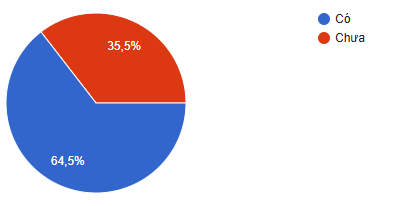
\includegraphics[width=0.6\textwidth]{assets/chart/1.4.5.png}
    \caption{\textit{Biểu đồ tỷ lệ sử dụng nền tảng đặt vé trực tuyến}} \textit{ 64.5\% cho biết đã từng sử dụng hình thức đặt vé trực tuyến.}
    \label{fig:muc_dich}
\end{figure}

    \begin{figure}[h]
    \centering
    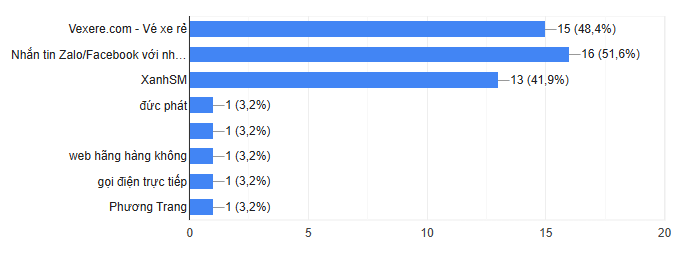
\includegraphics[width=0.8\textwidth]{assets/chart/1.4.6.png}
    \caption{\textit{Biểu đồ nền tảng hình thức đặt vé của người tham gia khảo sát.}} \textit{Trong đó nền tảng vé xe rẻ chiếm tới 48.4\%.}
    \label{fig:muc_xep_hang}
\end{figure}
\end{center}
% Kết quả về thói quen sử dụng và yếu tố ảnh hưởng
\subsubsection{Thói quen sử dụng và yếu tố ảnh hưởng}
\begin{itemize}
    \item \textbf{Lý do không sử dụng ứng dụng:} Những người không sử dụng ứng dụng đặt vé (35.5\%) cho biết họ ưu tiên đặt vé qua điện thoại hoặc trực tiếp tại quầy vì ``quen với cách truyền thống'' (51.6\%), ``không tin tưởng thông tin trên ứng dụng'' (19.4\%), hoặc ``muốn gọi điện cho chắc chắn'' (29\%).
    \item \textbf{Yếu tố quan trọng khi đặt vé trực tuyến:} Các yếu tố được người dùng đánh giá cao bao gồm (tỷ lệ tổng có thể hưn 100\%  do người dùng có thể chọn nhiều hơn 1 câu trả lời):
    \begin{itemize}
        \item Giao diện dễ hiểu và thân thiện (59.1\%),
        \item Có xác nhận sau mỗi bước (22.7\%),
        \item Bố cục rõ ràng theo thứ tự thao tác (54\%),
    \end{itemize}
    \item \textbf{Thiết bị sử dụng:} 90.9\% người tham gia cho biết họ sử dụng điện thoại di động để đặt vé, trong khi phần còn lại sử dụng máy tính xách tay hoặc máy tính bảng.
\end{itemize}

    \begin{figure}[h]
    \centering
    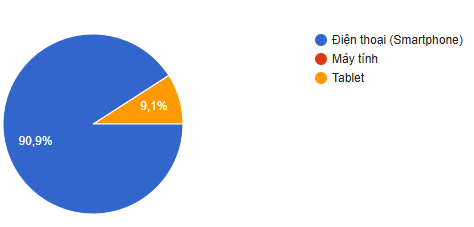
\includegraphics[width=0.6\textwidth]{assets/chart/1.4.8.png}
    \caption{\textit{Biểu đồ loại thiết bị đặt vé của người tham gia khảo sát.}} \textit{Trong đó điện thoại thông minh chiếm 90.9\%.}
    \label{fig:muc_xep_hang}
\end{figure}

% Kết quả về kỳ vọng và đề xuất từ người dùng
\subsubsection{Kỳ vọng và đề xuất từ người dùng}
\begin{figure}[h]
    \centering
    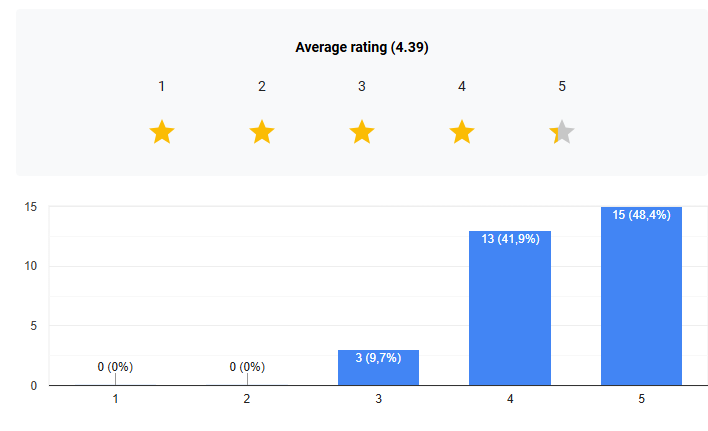
\includegraphics[width=0.8\textwidth]{assets/chart/1.4.7.png}
    \caption{\textit{Biểu đồ mục xếp hạng của người dùng cho các nền tảng đã sử dụng.}} \textit{ Vẫn tồn tại tỷ lệ đánh giá dưới 4 sao cao 9.7\%}
    \label{fig:muc_dich}
\end{figure}
\begin{itemize}
    \item \textbf{Tính năng mong muốn:} Người dùng kỳ vọng các tính năng sau trong một hệ thống đặt vé trực tuyến:
    \begin{itemize}
        \item Xem tuyến đường, giờ chạy và giá vé rõ ràng (77.3\%),
        \item Đánh giá và nhận xét nhà xe (54.45\%),
        \item Chọn ghế trực tiếp trên sơ đồ xe (81.8\%),
    \end{itemize}
    \item \textbf{Góp ý thiết kế giao diện:} Một số phản hồi mở đáng chú ý từ người dùng bao gồm:
    \begin{itemize}
        \item ``Ứng dụng nên thiết kế đơn giản, có thể xem nhanh giờ chạy của các nhà xe trước khi nhấn chi tiết.''
        \item ``Cần giao diện chọn ghế trực quan hơn, giống như khi đặt vé xem phim, để dễ hình dung vị trí.''
        \item ``Ứng dụng hiện tại hay bị lỗi, thông tin xe không load được, cần cải thiện tính ổn định.''
    \end{itemize}
\end{itemize}


% Kết luận về kết quả khảo sát

\section*{1.5 Phân tích nhu cầu người dùng}
Dựa trên dữ liệu khảo sát từ mục 1.4, nhóm nhận thấy người dùng đặt vé xe khách hiện nay gặp nhiều khó khăn do giao diện ứng dụng chưa tối ưu và thiếu các tính năng cần thiết. Báo cáo này phân tích chi tiết hành vi, vấn đề và nhu cầu của người dùng, từ đó đề xuất các giải pháp giao diện cụ thể nhằm cải thiện trải nghiệm đặt vé trên thiết bị di động.

\subsection*{1.5.1 Hành vi và thói quen người dùng}
Khảo sát cho thấy \textbf{90.9\% người dùng} sử dụng điện thoại thông minh để tra cứu và đặt vé xe khách, đặc biệt trong nhóm tuổi từ 18--25 (chiếm 51.6\% tổng số người tham gia khảo sát). Điều này nhấn mạnh tầm quan trọng của việc tối ưu giao diện cho thiết bị di động, với bố cục rõ ràng, phông chữ dễ đọc và thao tác cảm ứng mượt mà. Các yếu tố như kích thước nút bấm, khoảng cách giữa các thành phần giao diện và khả năng điều hướng nhanh là cần thiết để đảm bảo trải nghiệm tốt.

Xe khách là phương tiện di chuyển liên tỉnh phổ biến nhất, đặc biệt với nhóm người trẻ di chuyển để học tập, làm việc hoặc thăm gia đình. Tần suất di chuyển trung bình là \textbf{1 chuyến/tháng}, với các tuyến phổ biến là giữa các thành phố lớn.

Tuy nhiên, nhóm người dùng vẫn duy trì thói quen đặt vé truyền thống (gọi điện cho nhà xe hoặc mua trực tiếp tại bến) do:
\begin{itemize}
    \item \textbf{Thói quen lâu năm}: Đặc biệt ở nhóm tuổi trên 35, chiếm 3.2\% người khảo sát.
    \item \textbf{Thiếu niềm tin vào ứng dụng}: Lo ngại về tính minh bạch (giá vé, thông tin chuyến) và bảo mật thông tin cá nhân.
    \item \textbf{Khó khăn trong thao tác}: Một số người dùng lớn tuổi gặp khó khăn với giao diện phức tạp hoặc thiếu hướng dẫn rõ ràng.
\end{itemize}
Những yếu tố này cho thấy ứng dụng cần cung cấp thông tin minh bạch, dễ kiểm tra (ví dụ: giá vé, lịch sử đặt vé) và giao diện thân thiện để xây dựng niềm tin và khuyến khích người dùng chuyển từ phương thức truyền thống sang ứng dụng.

\subsection*{1.5.2 Các vấn đề người dùng thường gặp}
Qua khảo sát với \textbf{31 người dùng} từ các độ tuổi và khu vực khác nhau, nhóm ghi nhận các vấn đề chính sau ảnh hưởng đến trải nghiệm đặt vé:
\begin{enumerate}
    \item \textbf{Thông tin không rõ ràng} (báo cáo bởi 25.8\% người dùng):
    \begin{itemize}
        \item Nhiều ứng dụng không hiển thị đầy đủ hoặc rõ ràng các thông tin quan trọng như giờ khởi hành, thời gian di chuyển dự kiến, loại ghế (ghế ngồi, giường nằm), hoặc hãng xe.
        \item Người dùng phải thực hiện nhiều thao tác (nhấp qua nhiều màn hình) để tìm thông tin, gây mất thời gian và khó chịu.
        \item Một số ứng dụng không cập nhật trạng thái chuyến xe (hủy chuyến, thay đổi giờ) kịp thời.
    \end{itemize}
    \item \textbf{Giao diện phức tạp và khó sử dụng} (báo cáo bởi 45.2\% người dùng):
    \begin{itemize}
        \item Bố cục giao diện rối rắm, các nút bấm không rõ ràng hoặc quá nhỏ, đặc biệt trên màn hình di động.
        \item Quy trình đặt vé yêu cầu nhiều bước không cần thiết, như nhập lại thông tin đã lưu trước đó.
        \item Người dùng lớn tuổi (trên 35 tuổi) thường gặp khó khăn trong việc tìm kiếm chuyến xe hoặc chọn ghế.
    \end{itemize}
    \item \textbf{Không biết bước tiếp theo là gì} (chiếm 12.9\% người dùng):
    \begin{itemize}
        \item Không có sơ đồ ghế trực quan để chọn vị trí ngồi (tương tự hệ thống đặt vé xem phim).
        \item Thiếu chức năng đánh giá chất lượng nhà xe, khiến người dùng khó chọn được dịch vụ uy tín.
        \item Không hỗ trợ lưu vé điện tử hoặc gửi thông báo nhắc nhở trước giờ khởi hành.
        \item Thiếu bộ lọc nâng cao (ví dụ: lọc theo giá, loại xe, hoặc thời gian khởi hành).
    \end{itemize}
\end{enumerate}

\subsection*{1.5.3 Nhu cầu và mong muốn nổi bật}
Dựa trên phản hồi từ khảo sát và các câu hỏi mở, nhóm xác định các nhu cầu cốt lõi của người dùng và đề xuất giải pháp giao diện tương ứng:

\begin{table}[h]
\centering
\begin{tabular}{|p{4.5cm}|p{8.5cm}|}
\hline
\textbf{Nhu cầu người dùng} & \textbf{Giải pháp giao diện} \\
\hline
Giao diện rõ ràng, dễ hiểu & Thiết kế tối giản, hiển thị giờ khởi hành, giá vé, loại ghế ngay màn hình chính. \\
\hline
Tìm kiếm nhanh, ít thao tác & Thanh tìm kiếm với bộ lọc theo điểm đi/đến, thời gian, giá; gợi ý chuyến xe. \\
\hline
Chọn ghế trực quan & Sơ đồ ghế tương tác, hiển thị ghế trống/đã đặt, hỗ trợ phóng to/thu nhỏ. \\
\hline
Đặt vé nhanh chóng & Rút ngắn quy trình còn 3 bước, thông báo xác nhận rõ ràng. \\
\hline
Đánh giá chất lượng nhà xe & Tích hợp đánh giá sao, bình luận công khai từ người dùng trước. \\
\hline
Thông báo và lưu trữ vé & Lưu vé điện tử, gửi thông báo qua email/SMS trước giờ khởi hành. \\
\hline
\end{tabular}
\caption{\textit{Bảng tổng hợp nhu cầu người dùng và giải pháp giao diện.}}
\label{table2}
\end{table}

\subsection*{1.5.4 Định hướng thiết kế giao diện}
Dựa trên phân tích, nhóm đề xuất các định hướng thiết kế chính cho ứng dụng:
\begin{enumerate}
    \item \textbf{Tối ưu hóa cho thiết bị di động}: Đảm bảo giao diện tương thích với nhiều kích thước màn hình, ưu tiên điều hướng bằng một tay và thao tác cảm ứng mượt mà.
    \item \textbf{Minh bạch thông tin}: Hiển thị rõ ràng và đầy đủ các thông tin quan trọng (giờ, giá, loại xe, chính sách hủy vé) ngay từ màn hình đầu tiên.
    \item \textbf{Trải nghiệm liền mạch}: Giảm thiểu số bước thao tác, tích hợp các tính năng như lưu thông tin cá nhân, thanh toán nhanh qua ví điện tử, và thông báo tự động.
    \item \textbf{Thông báo rõ tiến trình đặt vé}: Đảm bảo người dùng dễ dàng biết được đã hoàn thành bao nhiêu \% và tiến trình còn lại bao nhiêu.
\end{enumerate}

Những định hướng này sẽ là cơ sở để phát triển một giao diện ứng dụng đáp ứng tốt nhu cầu người dùng, nâng cao trải nghiệm đặt vé và khuyến khích sử dụng phương thức đặt vé trực tuyến.



\section*{1.6 Tham khảo các hệ thống tương tự}
% Introducing the purpose of analyzing similar systems
Để hiểu rõ hơn về xu hướng thiết kế giao diện trong lĩnh vực đặt vé xe khách, nhóm đã khảo sát và phân tích các hệ thống phổ biến tại Việt Nam. Quá trình này giúp xác định các điểm mạnh cần học hỏi và những hạn chế cần khắc phục để thiết kế một giao diện mới tối ưu, đáp ứng tốt nhu cầu người dùng.

\subsection*{1.6.1 Hệ thống VeXeRe (\texttt{https://vexere.com})}
% Listing strengths and weaknesses of VeXeRe
\textbf{Ưu điểm:}
\begin{itemize}
    \item Cung cấp thông tin chuyến đi đầy đủ: giờ khởi hành, hãng xe, loại ghế (ghế ngồi, giường nằm), giá vé, điểm đón/trả.
    \item Tích hợp sơ đồ ghế trực quan, cho phép người dùng chọn vị trí trên xe dễ dàng.
    \item Hỗ trợ đa dạng phương thức thanh toán trực tuyến: thẻ ATM, ví điện tử, thẻ quốc tế.
    \item Hiển thị đánh giá và nhận xét từ người dùng trước, giúp tăng độ tin cậy.
\end{itemize}

\textbf{Hạn chế:}
\begin{itemize}
    \item Giao diện web trên thiết bị di động hơi rối, hiển thị đồng thời nhiều thông tin nhỏ (quảng cáo, khuyến mãi) gây khó theo dõi.
    \item Quy trình đặt vé dài (5--7 bước), đặc biệt với người dùng chưa đăng nhập, làm giảm trải nghiệm.
    \item Thiếu tính năng gợi ý tuyến đường dựa trên vị trí hiện tại hoặc lịch sử đặt vé của người dùng.
\end{itemize}

\subsection*{1.6.2 Website các hãng xe riêng (Thành Bưởi, Phương Trang, Hoàng Long)}
% Listing strengths and weaknesses of individual bus company websites
\textbf{Ưu điểm:}
\begin{itemize}
    \item Thiết kế đơn giản, phù hợp với người dùng quen thuộc với tuyến xe cố định (ví dụ: khách hàng trung thành của hãng).
    \item Cho phép đặt vé nhanh mà không cần tạo tài khoản.
\end{itemize}

\textbf{Hạn chế:}
\begin{itemize}
    \item Giao diện thiếu đồng bộ giữa các hãng; nhiều trang có thiết kế lỗi thời, không tối ưu cho thiết bị di động (chữ nhỏ, nút bấm khó thao tác).
    \item Thiếu sơ đồ chọn ghế trực quan; người dùng phải nhập thủ công hoặc chọn ngẫu nhiên.
    \item Không có chức năng lọc chuyến theo giờ, giá hoặc loại xe; tìm kiếm kém linh hoạt.
    \item Thiếu đánh giá chất lượng từ khách hàng trước, gây khó khăn trong việc chọn nhà xe uy tín.
\end{itemize}

\subsection*{1.6.3 Một số ứng dụng liên quan}

% Introducing the purpose of analyzing similar systems
Để khám phá các xu hướng thiết kế giao diện người dùng (UI) hiệu quả cho hệ thống đặt vé xe khách, nhóm đã nghiên cứu và phân tích các nền tảng phổ biến tại Việt Nam, bao gồm các hệ thống ngoài ngành vận tải như hệ thống rạp vé CGV (\texttt{https://www.cgv.vn}) và Medpro (\texttt{https://www.medpro.vn}). Phân tích này giúp nhận diện các điểm mạnh về thiết kế UI cần học hỏi và những hạn chế cần cải thiện, từ đó xây dựng một giao diện tối ưu, trực quan, và đáp ứng tốt nhu cầu người dùng. Qua đó, nhóm có đánh giá tổng quan về hai nền tảng này như sau:
\subsubsection*{- Hệ thống CGV (\texttt{https://www.cgv.vn})}
% Listing strengths and weaknesses of CGV
\textbf{Ưu điểm:}
\begin{itemize}
    \item Giao diện đơn giản, bố cục rõ ràng với thanh điều hướng cố định (``Lịch chiếu'', ``Phim'', ``Rạp''), giúp người dùng dễ dàng tìm kiếm thông tin.
    \item Sơ đồ chọn ghế trực quan, hiển thị dưới dạng bản đồ 2D với màu sắc tương phản (xanh cho ghế trống, đỏ/xám cho ghế đã đặt), hỗ trợ phóng to/thu nhỏ.
    \item Quy trình đặt vé tối ưu với 4--5 bước (chọn phim, rạp, suất chiếu, ghế, thanh toán), kèm nút kêu gọi hành động (CTA) nổi bật (màu đỏ/vàng).
    \item Tốc độ phản hồi nhanh, thao tác mượt mà, tối ưu cho cả máy tính và thiết bị di động.
    \item Hỗ trợ cá nhân hóa thông qua tài khoản thành viên (lưu lịch sử giao dịch, tích điểm) và tìm rạp gần nhất bằng GPS.
\end{itemize}

\noindent\textbf{Hạn chế:}
\begin{itemize}
    \item Giao diện có thể hiển thị quá nhiều quảng cáo hoặc khuyến mãi trên trang chủ, gây phân tâm cho người dùng.
    \item Tính năng gợi ý phim dựa trên sở thích hoặc lịch sử xem còn hạn chế, chưa thực sự cá nhân hóa sâu.
    \item Một số tính năng (như chọn ghế trên ứng dụng di động) có thể không ổn định khi tải đồng thời nhiều người dùng.
\end{itemize}

\subsubsection*{- Hệ thống MEDPRO (\texttt{https://www.medpro.vn})}
% Listing strengths and weaknesses of Medpro
\textbf{Ưu điểm:}
\begin{itemize}
    \item Thông tin được tổ chức rõ ràng theo khu vực, thời gian, bác sĩ; thanh tìm kiếm nổi bật hỗ trợ lọc chuyên khoa hoặc bệnh viện.
    \item Quy trình đặt lịch khám tối giản (tìm kiếm, chọn chuyên khoa, chọn giờ, xác nhận), với biểu mẫu chỉ yêu cầu thông tin cần thiết.
    \item Màu sắc nhẹ nhàng (xanh lam, trắng) tạo cảm giác tin cậy, phù hợp với lĩnh vực y tế; font chữ dễ đọc cho mọi lứa tuổi.
    \item Tính năng cá nhân hóa hiệu quả: lưu hồ sơ người dùng, gợi ý bác sĩ dựa trên lịch sử, và hỗ trợ tư vấn video từ xa.
    \item Hỗ trợ đa kênh (website, ứng dụng, tổng đài 1900 2115), đảm bảo giao diện responsive trên mọi thiết bị.
\end{itemize}

\noindent\textbf{Hạn chế:}
\begin{itemize}
    \item Giao diện trên thiết bị di động đôi khi tải chậm khi hiển thị danh sách bệnh viện hoặc bác sĩ dài.
    \item Thiếu đánh giá từ người dùng trước về bác sĩ hoặc cơ sở y tế, gây khó khăn trong việc lựa chọn.
    \item Một số tính năng nâng cao (như tư vấn video) yêu cầu đăng nhập, có thể làm gián đoạn trải nghiệm người dùng mới.
\end{itemize}
Giao diện của CGV và Medpro thể hiện sự cân bằng giữa tính trực quan, hiệu suất và cá nhân hóa. CGV nổi bật với sơ đồ ghế và quy trình đặt vé mượt mà, trong khi Medpro ghi điểm với tổ chức thông tin rõ ràng và tìm kiếm thông minh. Những yếu tố này cung cấp góc nhìn nhận quan trọng để thiết kế hệ thống đặt vé xe khách với giao diện đơn giản, dễ sử dụng và đáp ứng tốt nhu cầu người dùng.

\subsection*{1.6.4 Kinh nghiệm áp dụng cho hệ thống đặt vé xe khách}
% Summarizing lessons learned for bus ticket booking system
Dựa trên phân tích giao diện của CGV và MEDPRO, các bài học thiết kế UI sau có thể áp dụng để phát triển hệ thống đặt vé xe khách:
\begin{itemize}
    \item \textbf{Tối ưu hóa hành trình người dùng}: Thiết kế quy trình đặt vé với 4--5 bước (chọn tuyến đường, giờ khởi hành, ghế, thanh toán), sử dụng nút CTA nổi bật và hướng dẫn rõ ràng để giảm thiểu sai sót.
    \item \textbf{Tính trực quan}: Áp dụng sơ đồ ghế trực quan như CGV, với màu sắc chủ đạo (cam, trắng, đen) và khả năng phóng to/thu nhỏ. Tổ chức thông tin tuyến xe theo khu vực, thời gian như Medpro.
    \item \textbf{Màu sắc và typography}: Sử dụng bảng màu đơn giản chỉ gồm màu chủ đạo và font chữ sans-serif dễ đọc, phù hợp với nhiều đối tượng, đặc biệt người lớn tuổi.
    \item \textbf{Tương tác}: Thao tác mượt mà, hiệu ứng hover hoặc chuyển đổi nhẹ nhàng tăng tính thân thiện.
    \item \textbf{Cá nhân hóa}: Tích hợp tài khoản người dùng để lưu lịch sử đặt vé, gợi ý chuyến xe và cung cấp thông báo thời gian thực về trạng thái vé.
    \item \textbf{Tương thích đa nền tảng}: Thiết kế giao diện responsive đảm bảo trải nghiệm nhất quán.
\end{itemize}



% Summarizing design principles in a table
\noindent Dựa trên phân tích các hệ thống trên, nhóm đề xuất các nguyên tắc thiết kế quan trọng nhất cho giao diện ứng dụng:

\begin{table}[h]
\centering
\begin{tabular}{|p{4.5cm}|p{8.5cm}|}
\hline
\textbf{Nguyên tắc thiết kế} & \textbf{Ý nghĩa cụ thể} \\
\hline
Hiển thị thông tin quan trọng & Hiển thị giá vé, giờ khởi hành, loại xe, ghế trống ngay màn hình chính. \\
\hline
Tối ưu thao tác đặt vé & Giảm quy trình còn 4--5 bước, đảm bảo xác nhận rõ ràng sau mỗi thao tác. \\
\hline
Giao diện tương thích di động & Thiết kế responsive, ưu tiên nút bấm lớn, điều hướng bằng một tay. \\
\hline
Chọn ghế trực quan & Cung cấp sơ đồ ghế tương tác, dễ phóng to/thu nhỏ, xác nhận tức thì. \\
\hline
Xây dựng niềm tin & Hiển thị đánh giá nhà xe, thông tin xác nhận vé. \\
\hline
\end{tabular}
\caption{\textit{Nguyên tắc thiết kế giao diện ứng dụng đặt vé xe khách}}
\label{table3}
\end{table}

Những nguyên tắc này sẽ định hướng thiết kế một giao diện thân thiện, hiệu quả, đáp ứng tốt nhu cầu người dùng và khắc phục các hạn chế của các hệ thống hiện tại.

\section*{1.7 Tổng kết chương}
% Summarizing the chapter's key findings and purpose
Trong chương này, nhóm đã thực hiện khảo sát, phân tích nhu cầu người dùng và tham khảo các hệ thống đặt vé xe khách hiện hành để xây dựng cơ sở cho việc thiết kế giao diện ứng dụng. Các hoạt động này giúp nhóm nhận diện những vấn đề cốt lõi và xác định định hướng phát triển, bao gồm:

\begin{itemize}
    \item \textbf{Giao diện chưa tối ưu}: Nhiều ứng dụng hiện nay có bố cục phức tạp, thiếu trực quan và không thân thiện với người dùng mới.
    \item \textbf{Nhu cầu người dùng}: Người dùng mong muốn một hệ thống đặt vé minh bạch về thông tin (giá vé, giờ khởi hành, loại xe), thao tác đơn giản và hỗ trợ chọn ghế trực quan, tương tự hệ thống đặt vé xem phim.
    \item \textbf{Tầm quan trọng của thiết bị di động}: Với 90.9\% người dùng sử dụng điện thoại thông minh để đặt vé, giao diện cần được thiết kế \textit{responsive}, ưu tiên thao tác một tay, nút bấm lớn và điều hướng mượt mà.
\end{itemize}

% Highlighting insights from system analysis
Việc tham khảo các nền tảng như VeXeRe và các ứng dụng ngoài ngành (CGV, MEDPRO) đã cung cấp nhiều bài học thiết kế thực tiễn, bao gồm cách tổ chức thông tin, tối ưu quy trình đặt vé và xây dựng niềm tin với người dùng. Những kết quả từ khảo sát và phân tích này sẽ là cơ sở để xác định yêu cầu chức năng, thiết kế giao diện và phát triển hệ thống trong các chương tiếp theo, đảm bảo ứng dụng đáp ứng tốt nhu cầu của người dùng ở mọi lứa tuổi.